\documentclass{article}
%%% INICIO DEL PREÁMBULO %%%

\usepackage[greek,spanish,es-tabla,es-nodecimaldot,es-noindentfirst]{babel}
\usepackage{fontspec}
\setmonofont{Consolas Bold}
\usepackage{babelbib}
\usepackage{nccmath}
\usepackage[oldvoltagedirection]{circuitikz}
\usepackage{amsthm}
\usepackage{lipsum}
\usepackage{tcolorbox}
\usepackage[thicklines]{cancel}
\usepackage{mathtools}
\usepackage{amssymb}
\usepackage{amsmath}
\usepackage[listformat=empty]{caption}
\captionsetup{
         listformat=empty,
         justification=justified,
		 font=Large
}
\usepackage[titles]{tocloft}
\cftsetindents{figure}{0em}{1.5em}
\renewcommand{\cftdot}{}

\usepackage{subcaption}   
\usepackage{color}       
\usepackage{verbatim}     
\usepackage{enumerate}
\usepackage{geometry} 
\geometry{a4paper,left=35mm,right=35mm,top=15mm,bottom=15mm}
\usepackage{isotope}
\usepackage{maybemath} 
\usepackage{upgreek}
\usepackage{wasysym} 
\usepackage[italic]{hepparticles}
\usepackage{subdepth}
\usepackage[italicdiff]{physics}
\usepackage{braket}
\usepackage{tensor}
\usepackage{chemformula} 
\usepackage{tikz} \usetikzlibrary{babel}
\usepackage{siunitx}
\usepackage{url}
\usepackage{listings}
\usepackage{multirow}
\usepackage{multicol}
\usepackage[colorlinks=true]{hyperref}
\hypersetup{
citecolor = blue,
linkcolor = blue,
urlcolor = blue,
pdfauthor = {Javier Rodrigo López}
}
\usepackage{eso-pic}
\usepackage{siunitx}
\sisetup{
round-mode      = places,
round-precision = 2,
}

% tikz
\usepackage{tikz} \usetikzlibrary{fit,babel,shapes,arrows,positioning}
\tikzstyle{block} = [draw, fill=white, rectangle, 
    minimum height=3em, minimum width=6em]
\tikzstyle{sum} = [draw, fill=white, circle, node distance=1cm]
\tikzstyle{input} = [coordinate]
\tikzstyle{output} = [coordinate]
\tikzstyle{pinstyle} = [pin edge={to-,thin,black}]
\tikzset{
block/.style = {draw, fill=white, rectangle, minimum height=3em, minimum width=3em},
tmp/.style  = {coordinate}, 
sum/.style= {draw, fill=white, circle, node distance=1cm},
input/.style = {coordinate},
output/.style= {coordinate},
pinstyle/.style = {pin edge={to-,thin,black}}
}

% Títulos
\usepackage{titlesec}
\titleformat{\section}
	{\normalfont\Large\bfseries}{\thesection}{1em}{}[{\titlerule[0.8pt]}]
\titleformat{\subsubsection}
	{\normalfont\normalsize\bfseries}{\thesubsubsection}{1em}{}[{\titlerule[0.05pt]}]
\titlespacing{\section}{0pt}{2\parskip}{\parskip}
\titlespacing{\subsection}{0pt}{\parskip}{0pt}
\titlespacing{\subsubsection}{0pt}{\parskip}{0pt}

% Numeración de secciones
\setcounter{tocdepth}{2}
\setcounter{secnumdepth}{2}

% Enumerations
\newcounter{myenumi}
\renewcommand{\themyenumi}{\alph{myenumi})}
\newenvironment{myenumerate}{\setlength{\parindent}{0pt}\setcounter{myenumi}{0}\renewcommand{\item}{\par\refstepcounter{myenumi}\makebox[1.3em][l]{\themyenumi}}}{\par\bigskip\noindent\ignorespacesafterend}

% Organización del texto
\newcommand{\formula}[1]{\vspace{13 pt}\noindent \textbf{\underline{#1}}}
\newcommand{\subtext}[1]{_{\text{#1}}}

% Unidades y utilidades varias
\renewcommand{\S}{\operatorname{S}}
\newcommand{\dB}{\operatorname{dB}}
\newcommand{\dBW}{\operatorname{dBW}}
\newcommand{\dBm}{\operatorname{dBm}}
\newcommand{\Hz}{\operatorname{Hz}}
\newcommand{\s}{\operatorname{s}}
\newcommand{\A}{\operatorname{A}}
\newcommand{\V}{\operatorname{V}}
\newcommand{\ohm}{\,\Omega}
\newcommand{\Pa}{\operatorname{Pa}}
\newcommand{\W}{\operatorname{W}}
\newcommand{\I}{\operatorname{I}}
\newcommand{\K}{\operatorname{K}}
\newcommand{\m}{\operatorname{m}}
\newcommand{\mm}{\operatorname{mm}}
\newcommand{\rad}{\operatorname{rad}}
\newcommand{\mol}{\operatorname{mol}}
\newcommand{\J}{\operatorname{J}}
\newcommand{\kg}{\operatorname{kg}}
\newcommand{\incremento}{\Delta}
\newcommand{\psus}{\, \ldots \,}
\newcommand{\sen}{\operatorname{\sen}}
\renewcommand{\sin}{\sen}
\renewcommand{\arcsin}{\arcsen}
\renewcommand{\arctan}{\arctg}
\renewcommand{\min}{\operatorname{mín}}

\definecolor{mygreen}{RGB}{28,172,0} % color values Red, Green, Blue
\definecolor{mylilas}{RGB}{170,55,241}

\lstset{language=Matlab,
	numbers=none,
    breaklines=true,
    morekeywords={matlab2tikz},
    keywordstyle=\color{blue},
    morekeywords=[2]{1}, keywordstyle=[2]{\color{black}},
    identifierstyle=\color{black},
    stringstyle=\color{mylilas},
    commentstyle=\color{mygreen},
	showspaces=false,
    showstringspaces=false,
    numberstyle={\tiny \color{black}},
    numbersep=9pt,
    emph=[1]{for,end,break},emphstyle=[1]\color{red},
	escapeinside={\%*}{*)},
	basicstyle=\footnotesize\ttfamily,
	columns=flexible
}

% Vectores
\usepackage[c]{esvect}
\renewcommand{\vec}[1]{\vv{{#1}}}
\newcommand{\proy}[2]{\operatorname{proy}_{\vec{#2}}\vec{#1}}
\newcommand{\antiparallel}{\downharpoonleft \! \upharpoonright}
\newcommand{\parallelvec}{\upharpoonleft \! \upharpoonright}

% Espaciado
\usepackage{enumitem}
\setlist{before={\parskip=3pt}, after=\vspace{\baselineskip}}
\setlength{\parindent}{0pt}
\setlength{\parskip}{0.5em}

% Estadística
\DeclareMathOperator{\Var}{Var}
\DeclareMathOperator{\Cov}{Cov}
\renewcommand{\var}{\sigma ^2}
\DeclareMathOperator{\B}{B}
\DeclareMathOperator{\BN}{BN}
\DeclareMathOperator{\Geo}{Geo}
\DeclareMathOperator{\Poisson}{Poisson}
\DeclareMathOperator{\Exp}{Exp}
\DeclareMathOperator{\N}{N}
\DeclareMathOperator{\Mult}{Mult}
\newcommand{\probCond}[2]{P \left( #1 \: \middle\vert\:  #2 \right) }

% Electromagnetismo y Ondas
\newcommand{\errorGrave}{\textbf{FG!!!}}
\newcommand{\mas}{M.A.S.}
\newcommand{\mcu}{M.C.U.}
\newcommand{\ed}{E.D.}
\newcommand{\edmas}{E.D. del M.A.S.}
\usepackage{esint}

% Señales y Sistemas
\renewcommand{\H}{H}

% Circled number
\newcommand{\circledNumber}[1]{\raisebox{.9pt}{\textcircled{\raisebox{-.9pt}{#1}}}}

% Footnotes
% \renewcommand{\thefootnote}{\fnsymbol{footnote}}

%%% FIN DEL PREÁMBULO %%%

% Título y portada
\title{\Huge Informe Práctica 2\\\vspace*{5pt}
\Large Señales y Sistenas}
\author{Javier Rodrigo López \thanks{Correo electrónico: \href{mailto:javier.rlopez@alumnos.upm.es}{\texttt{javier.rlopez@alumnos.upm.es}}}} 
\date{\today}

%%% INICIO DEL DOCUMENTO %%%
\begin{document}

\maketitle

\tableofcontents
\setlength{\cftparskip}{0.5\baselineskip}
\listoffigures

\newpage

\section{Introducción}
Las figuras que se adjuntan aparecen en el mismo orden en el cual son generadas al ejecutar el script de MATLAB. En el título de cada figura aparece el apartado al que pertenece.

Es aconsejable mirar el código para entender qué gráfica se genera en cada apartado y a qué ejercicio corresponde con mayor facilidad.

\newpage

\section{Código}
\pagestyle{empty}
\begin{lstlisting}
	% Autor: Javier Rodrigo López
	% Laboratorio de Señales y Sistemas - Práctica 2
	% Fecha de finalización: 16/03/2021
	%
	% Para visualizar esta práctica, se ha implementado la función 'pause',
	% por lo que durante la ejecución cada gráfica se generará al pulsar la
	% tecla Enter. La última vez que sea pulsada, cerrará todas las ventanas.
	
	%% Preámbulo
	% Comandos útiles
	clear all
	clc
	close all
	
	% Definición de señales impulso y escalón
	d = @(t) t == 0;
	u = @(t) t >= 0;
	
	% Constantes
	A1 = 2;
	A2 = -2;
	A3 = 3;
	A4 = -1/2;
	N1 = 6;
	N2 = 4;
	N3 = 3;
	N4 = 2;
	N5 = 20;
	N6 = 12;
	W1 = 1/3;
	W2 = 3 * pi / 8;
	
	%% Ejercicio 1
	% Suficientes muestras para representar todas las señales.
	n = -10:10;
	
	% Definición de las señales con las que trabajaremos.
	x1 = @(n) A1 * (u(n + N1) - u(n - N1));
	x2 = @(n) A2 .* u(n + N2) .* u(-n + N2);
	x3 = @(n) A3 * (u(n + N1) - u(n - N2)) .* exp(1i * W1 .* n);
	
	figure
	stem(n, x1(n)), title('1 - Señal x_1[n]'), xlabel('n')
	pause
	figure
	stem(n, x2(n)), title('1 - Señal x_2[n]'), xlabel('n')
	pause
	figure
	subplot(2, 1, 1)
	stem(n, real(x3(n))), title('1 - Señal x_3[n]'), ylabel('Parte real')
	subplot(2, 1, 2)
	stem(n, imag(x3(n))), ylabel('Parte imaginaria'), xlabel('n')
	pause
	
	% Cálculo de las convoluciones.
	[y1, n1] = convolucion(x1(n), x1(n + N3), n);
	[y2, n2] = convolucion(x1(n), x2(n), n);
	[y3, n3] = convolucion(x1(n), y2, n);
	[y4, n4] = convolucion(real(x3(n)), imag(x3(n - N4)), n);
	
	% Recorte de las señales, para mejor representación.
	y1 = y1(1, 1:find(y1, 1, 'last'));
	n1 = n1(1:length(y1));
	
	y2 = y2(1, 1:find(y2, 1, 'last'));
	n2 = n2(1:length(y2));
	
	y3 = y3(1, 1:find(y3, 1, 'last'));
	n3 = n3(1:length(y3));
	
	y4 = y4(1, 1:find(y4, 1, 'last'));
	n4 = n4(1:length(y4));
	
	% Ajuste de los límites para que las señales se ajusten al ancho de la
	% gráfica.
	figure
	stem(n1, y1), title('1.1 - Señal y_1[n]'), xlabel('n'), axis tight
	pause
	figure
	stem(n2, y2), title('1.2 - Señal y_2[n]'), xlabel('n'), axis tight
	pause
	figure
	stem(n3, y3), title('1.3 - Señal y_3[n]'), xlabel('n'), axis tight
	pause
	figure
	stem(n4, y4), title('1.4 - Señal y_4[n]'), xlabel('n'), axis tight
	pause
	
	%% Ejercicio 2
	n = 0:N5;
	imp = d(n);
	
	% Apartado 2.1
	a1 = [1 0 0 0];
	b1 = [A1 0 0 A3];
	
	h1 = filter(b1, a1, imp);
	
	figure
	stem(n, h1), title('2.1 - Señal h1[n]'), xlabel('n')
	pause
	
	% Resultado: Este sistema es estable, pues su respuesta al impulso es una
	% combinación de dos deltas. La suma absoluta de todos sus valores es un
	% valor finito.
	
	% Apartado 2.2
	a2 = [1 1 0 0];
	b2 = [1 A1 A2 A3];
	
	h2 = filter(b2, a2, imp);
	
	figure
	stem(n, h2), title('2.2 - Señal h2[n]'), xlabel('n')
	pause
	
	% Resultado: Este sistema no es estable. Si realizamos la suma absoluta de
	% todos sus valores, esta tiende a infinito.
	
	%% Ejercicio 3
	x4 = A1 * (u(n) - u(n - N1));
	x5 = A3 * exp(1i * W1 * n) .* u(n);
	
	% Apartado 3.1
	[y41, ~] = convolucion(x4, h1, n);
	y41 = y41(1, 1:length(n));
	y41f = filter(b1, a1, x4);
	
	figure
	subplot(2, 1, 1)
	stem(n, y41), title('3.1 - Señal y_4_1[n] - convolucion()')
	subplot(2, 1, 2)
	stem(n, y41f), title('3.1 - Señal y_4_1[n] - filter()'), xlabel('n')
	pause
	
	[y42, ~] = convolucion(x4, h2, n);
	y42 = y42(1, 1:length(n));
	y42f = filter(b2, a2, x4);
	
	figure
	subplot(2, 1, 1)
	stem(n, y42), title('3.1 - Señal y_4_2[n] - convolucion()')
	subplot(2, 1, 2)
	stem(n, y42f), title('3.1 - Señal y_4_2[n] - filter()'), xlabel('n')
	pause
	
	% Apartado 3.2
	[y51, ~] = convolucion(x5, h1, n);
	y51 = y51(1, 1:length(n));
	y51f = filter(b1, a1, x5);
	
	figure
	subplot(2, 2, 1)
	stem(n, real(y51)), title('3.2 - Señal y_5_1[n] - convolucion()'), ylabel('Parte real')
	subplot(2, 2, 3)
	stem(n, imag(y51)), xlabel('n'), ylabel('Parte imaginaria')
	subplot(2, 2, 2)
	stem(n, real(y51f)), title('3.2 - Señal y_5_1[n] - filter()'), ylabel('Parte real')
	subplot(2, 2, 4)
	stem(n, imag(y51f)), xlabel('n'), ylabel('Parte imaginaria')
	pause
	
	[y52, ~] = convolucion(x5, h2, n);
	y52 = y52(1, 1:length(n));
	y52f = filter(b2, a2, x5);
	
	figure
	subplot(2, 2, 1)
	stem(n, real(y52)), title('3.2 - Señal y_5_2[n] - convolucion()'), ylabel('Parte real')
	subplot(2, 2, 3)
	stem(n, imag(y52)), xlabel('n'), ylabel('Parte imaginaria')
	subplot(2, 2, 2)
	stem(n, real(y52f)), title('3.2 - Señal y_5_2[n] - filter()'), ylabel('Parte real')
	subplot(2, 2, 4)
	stem(n, imag(y52f)), xlabel('n'), ylabel('Parte imaginaria')
	pause
	
	% Resultados: Ambas gráficas son iguales, independientemente de la función
	% utilizada. Podemos suponer que los resultados son correctos.
	
	%% Ejercicio 4
	n = 0:15;
	x = A1 * cos(W2 * n) .* (u(n) - u(n - N6));
	imp = d(n);
	
	% Cálculo de las señales solicitadas.
	a = [1 0 A4];
	b = [0 0 A1];
	s = filter(b, a, x);
	
	h = d(n) + A1 * d(n - N4) + A2 * d(n - N2) +A3 * d(n - N1);
	[v, ~] = convolucion(h, s, n);
	v = v(1, 1:length(n));
	
	y = v + s .* cos(pi * n / 2);
	
	figure
	stem(n, s), title('4 - Señal s[n]'), xlabel('n')
	pause
	figure
	stem(n, v), title('4 - Señal v[n]'), xlabel('n')
	pause
	figure
	stem(n, y), title('4 - Señal y[n]'), xlabel('n')
	pause
	
	close all
	
	%% Funciones
	
	% Realiza la convolución mediante la función 'conv()'.
	function [y, eje] = convolucion(x, h, eje)
		% Cálculo de los instantes iniciales.
		xi = find(x, 1) + eje(1, 1) - 1;
		hi = find(h, 1) + eje(1, 1) - 1;
		yi = xi + hi;
	
		% Hacemos que los vectores empiecen desde el primer valor no nulo.
		x = x(1, find(x, 1):end);
		h = h(1, find(h, 1):end);
	
		% Calculamos el resultado y su eje de tiempos.
		y = conv(x, h);
		eje = (1:length(y)) + yi - 1;
	end
	

\end{lstlisting}

\newpage
\pagestyle{plain}
\section{Figuras}

\begin{figure}[h] \caption[Figura 1]{}
	\centering
	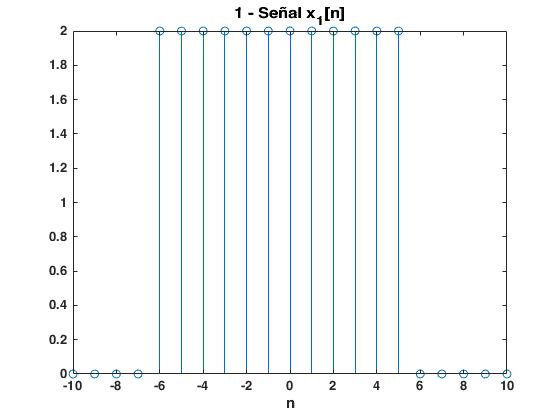
\includegraphics[width=\linewidth]{./Figures/01.png}
\end{figure}

\begin{figure}[h!] \caption[Figura 2]{}
	\centering
	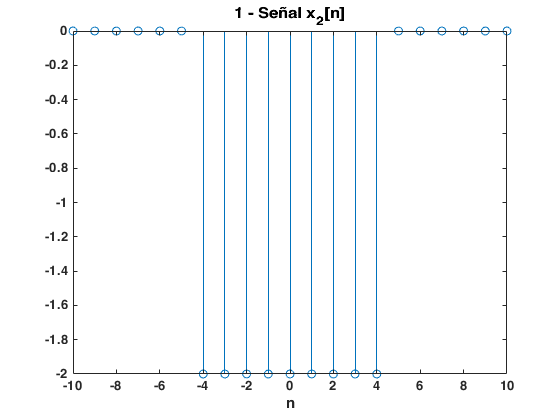
\includegraphics[width=\linewidth]{./Figures/02.png}
\end{figure}

\begin{figure} \caption[Figura 3]{}
	\centering
	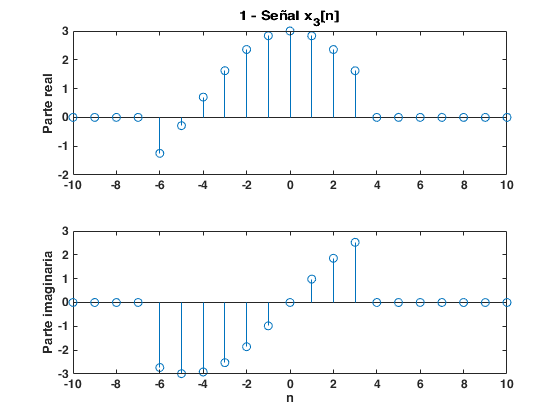
\includegraphics[width=\linewidth]{./Figures/03.png}
\end{figure}

\begin{figure} \caption[Figura 4]{}
	\centering
	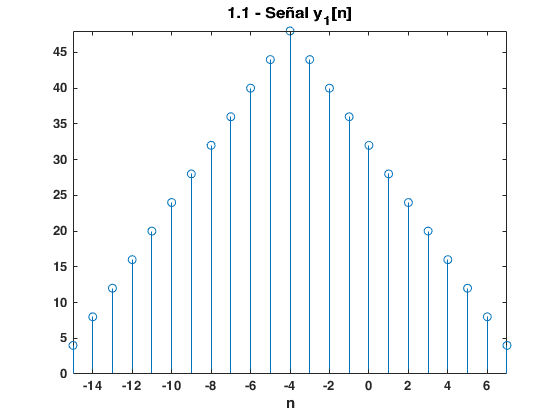
\includegraphics[width=\linewidth]{./Figures/04.png}
\end{figure}

\begin{figure} \caption[Figura 5]{}
	\centering
	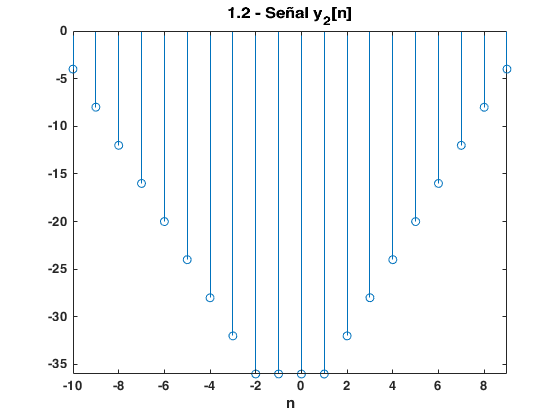
\includegraphics[width=\linewidth]{./Figures/05.png}
\end{figure}

\begin{figure} \caption[Figura 6]{}
	\centering
	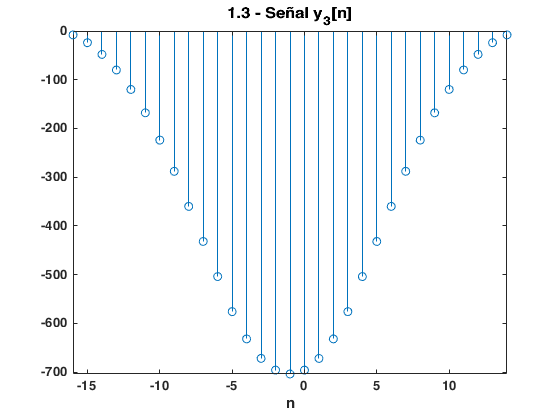
\includegraphics[width=\linewidth]{./Figures/06.png}
\end{figure}

\begin{figure} \caption[Figura 7]{}
	\centering
	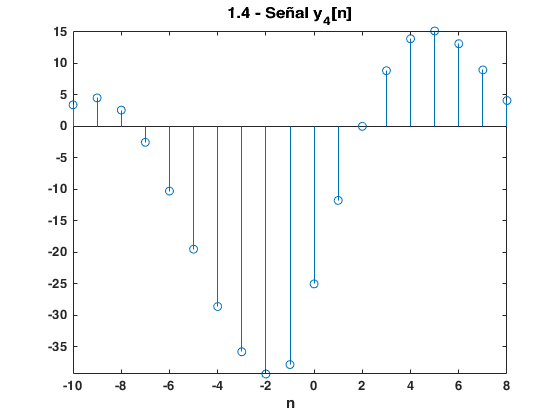
\includegraphics[width=\linewidth]{./Figures/07.png}
\end{figure}

\begin{figure} \caption[Figura 8]{}
	\centering
	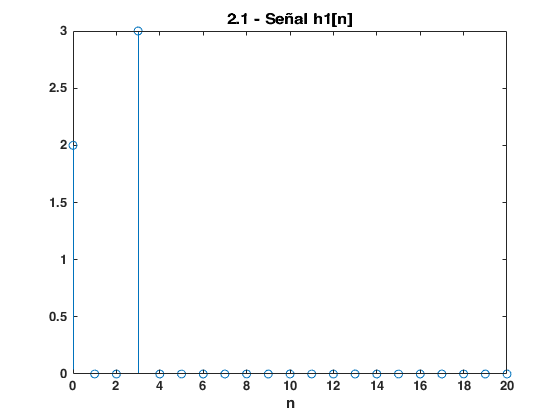
\includegraphics[width=\linewidth]{./Figures/08.png}
\end{figure}

\begin{figure} \caption[Figura 9]{}
	\centering
	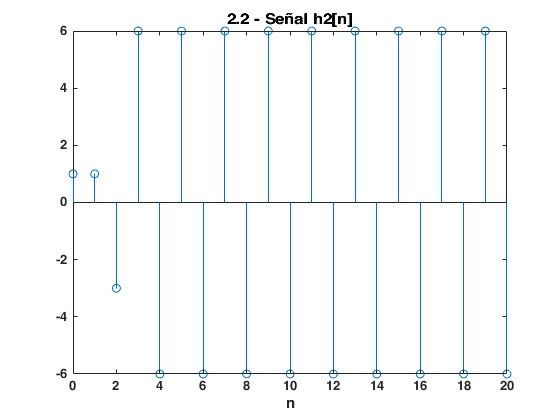
\includegraphics[width=\linewidth]{./Figures/09.png}
\end{figure}

\begin{figure} \caption[Figura 10]{}
	\centering
	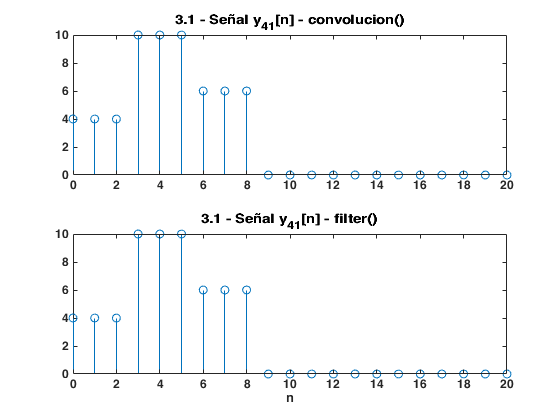
\includegraphics[width=\linewidth]{./Figures/10.png}
\end{figure}

\begin{figure} \caption[Figura 11]{}
	\centering
	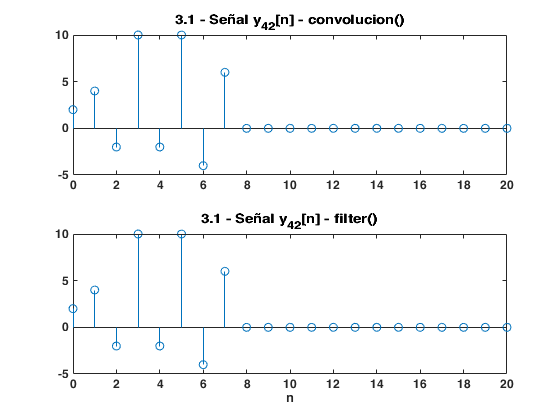
\includegraphics[width=\linewidth]{./Figures/11.png}
\end{figure}

\begin{figure} \caption[Figura 12]{}
	\centering
	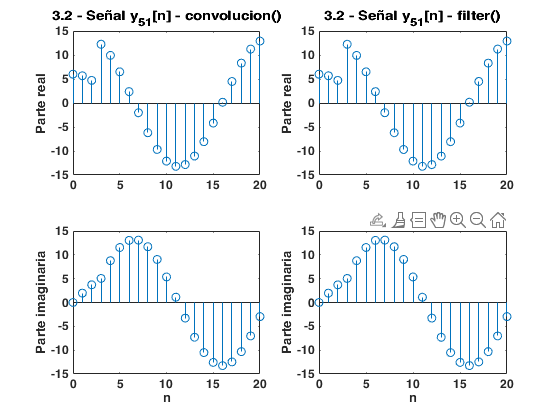
\includegraphics[width=\linewidth]{./Figures/12.png}
\end{figure}

\begin{figure} \caption[Figura 13]{}
	\centering
	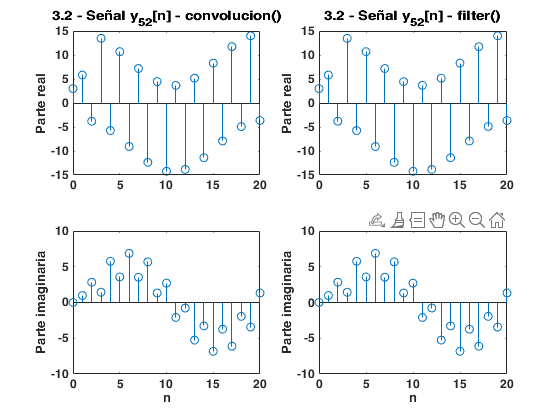
\includegraphics[width=\linewidth]{./Figures/13.png}
\end{figure}

\begin{figure} \caption[Figura 14]{}
	\centering
	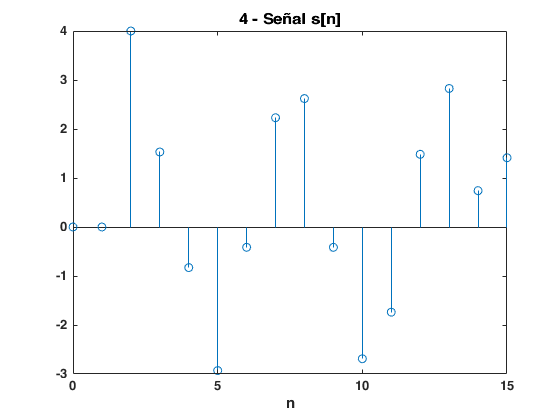
\includegraphics[width=\linewidth]{./Figures/14.png}
\end{figure}

\begin{figure} \caption[Figura 15]{}
	\centering
	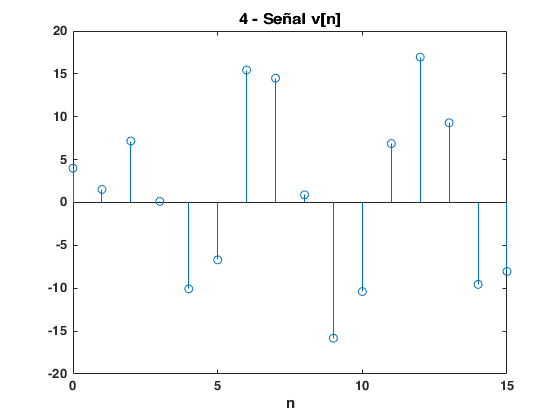
\includegraphics[width=\linewidth]{./Figures/15.png}
\end{figure}

\begin{figure} \caption[Figura 16]{}
	\centering
	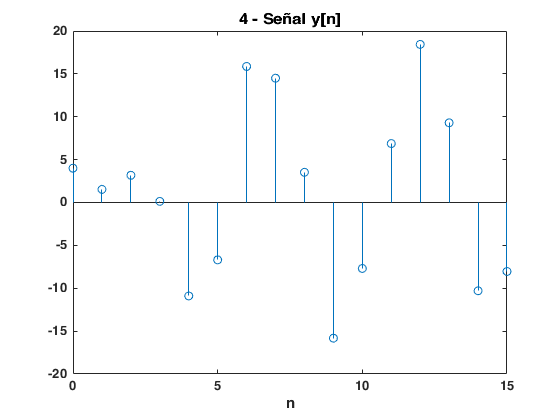
\includegraphics[width=\linewidth]{./Figures/16.png}
\end{figure}

\end{document}